\documentclass[20pt]{article}
\usepackage[latin1]{inputenc}
\usepackage{epsf}
\usepackage{graphicx,psfrag,color,pstcol,pst-grad}
\usepackage{pst-blur}
\usepackage{amsmath,amssymb}
\usepackage{latexsym}
\usepackage{calc}
\usepackage{multicol,xspace}
\usepackage{verbatim} % for comment

\graphicspath{{.}{inclposter-2007/}{images/}}  
% defines the width and height of the poster, scaled down to a viewable size
%\def\width{12in}  % this is 3'/3 = 36'' / 3 = 12''
%\def\height{17in} % this is 4'/3 = 48'' / 3 = 16''+ 3'/3 (for top and bottom inch)
%A1:
% size: 59.4cm wide x 84 cm high (A1)
% (23.5 inches x 33 inches)
%A2:
% size: 42 cm wide x 59.4 cm high (A2)
% (16.5 inches x 23.5 inches)
\def\width{42cm}  % this is 3'/3 = 36'' / 3 = 12''
\def\height{59.4cm} % this is 4'/3 = 48'' / 3 = 16''+ 3'/3 (for top and bottom inch)

% Set paper format
\setlength{\paperwidth}{\width}
\setlength{\paperheight}{\height}
\special{papersize=\width,\height}
\pagestyle{empty}

% width of colored background
\newlength{\bgwidth}
%\setlength{\bgwidth}{12in}
\setlength{\bgwidth}{42cm}
% height of colored background
\newlength{\bgheight}
%\setlength{\bgheight}{16.3in}
\setlength{\bgheight}{58cm}

% Removing all margins and spacing
\setlength{\topmargin}{-0.5in}
%\setlength{\topmargin}{0.3in}
\setlength{\headheight}{0in}
\setlength{\headsep}{0in}
\setlength{\topskip}{0in}
\setlength{\footskip}{0in}
\setlength{\oddsidemargin}{-0.45in}
%\setlength{\parindent}{0em}
%\setlength{\parskip}{5cm}
%\setlength{\itemsep}{0.1cm}
%\setlength{\parsep}{0.1cm}

% Set textwidth to leave 1 inch on each side
\setlength{\textwidth}{\paperwidth}
\addtolength{\textwidth}{-1.0in}
\setlength{\textheight}{\paperheight}
\addtolength{\textheight}{-0.3in}


% The white box where the text is
\newsavebox{\dummybox}
\newenvironment{textbox}
{\begin{lrbox}{\dummybox}\begin{minipage}{0.9\columnwidth}}
{\end{minipage}\end{lrbox}\raisebox{-\depth}{\psshadowbox[framesep=1em,framearc=.1,shadow=true]{\usebox{\dummybox}}}\vspace{0.005\textheight}}


% Colors for the sections and subsections
%\definecolor{udsect}{rgb}{0 ,0 ,1}
%\definecolor{udsubsect}{rgb}{0, 0.5, 0}
\definecolor{udsect}{rgb}{0.0, 0.4, 0.27}
\definecolor{udsubsect}{rgb}{0.0, 0.4, 0.27}

\newcommand{\masyv}{\texttt{MASyV}\xspace}
\newcommand{\cimmsim}{\texttt{CImmSim}\xspace}
\newcommand{\maimmune}{\texttt{ma\_immune}\xspace}
\begin{document}
\huge
\begin{center}


%%%%%%%%%%%%%%%%%%%%%%%%%%%%%%%%%%%%%%%%%%%%%%%%%%%%%%%%%%%%%%%%%%%%%%%%%%%%%%%%%%%
%                                    Background                                   %
%%%%%%%%%%%%%%%%%%%%%%%%%%%%%%%%%%%%%%%%%%%%%%%%%%%%%%%%%%%%%%%%%%%%%%%%%%%%%%%%%%%
%\newrgbcolor{gradbegin}{1 0.82 0.16}
%\newrgbcolor{gradend}{0.0 0.4 0.27}
%\psframe[linestyle=none,fillstyle=solid,fillcolor=gradbegin](-0.5\bgwidth,1.6in)(0.5\bgwidth,-0.5\bgheight)
%\psframe[linestyle=none,fillstyle=gradient,gradbegin=gradbegin,gradend=gradend,gradmidpoint=1](-0.5\bgwidth,-0.35\bgheight)(0.5\bgwidth,-0.45\bgheight)
%\psframe[linecolor=gradend,fillstyle=solid,fillcolor=gradend](-0.5\bgwidth,-0.4489\bgheight)(0.5\bgwidth,-\bgheight)

%%%%%%%%%%%%%%%%%%%%%%%%%%%%%%%%%%%%%%%%%%%%%%%%%%%%%%%%%%%%%%%%%%%%%%%%%%%%%%%%%%%
%                                     Header                                      %
%%%%%%%%%%%%%%%%%%%%%%%%%%%%%%%%%%%%%%%%%%%%%%%%%%%%%%%%%%%%%%%%%%%%%%%%%%%%%%%%%%%
\vspace{-2.0cm}
%\psbox[fillstyle=solid,linewidth=1pt,framearc=.5]{\makebox[0.98\textwidth]{
	\parbox[c]{1.4cm}{
\includegraphics[width=3.8cm]{images/hiplogo.eps}}
	\hspace{0.6cm}
   \parbox[c]{0.8\linewidth}{
		\begin{center}

			\textbf{\Huge INCL/ABLA INTRA-NUCLEAR CASCADE MODELS \\ IN {\sf GEANT4~9.2}} \\[0.5em]
			\textbf{\LARGE Aatos Heikkinen$^{1}$, \underline{Pekka Kaitaniemi}$^{\dagger, 1, 2}$} \\[0.3em]
			{\Large $^{\dagger}$ {\tt pekka.kaitaniemi@cea.fr}} \\
                        {\LARGE $^1$~Helsinki Institute of Physics, P.O.B. 64, FIN-00014 University of Helsinki, Finland}\\
                        {\LARGE $^2$~CEN-Saclay, CEA-IRFU/SPhN, 91 191 Gif sur Yvette, France}
                        \vskip2cm
		\end{center}
	}
	\parbox[c]{5.3cm}{\hspace{-1.0cm} 
\includegraphics[width=5.6cm]{images/g4logo.eps}}
%}}
% Helsinki Institute of Physics, P.O.B. 64, FIN-00014 University of Helsinki, Finland
% email: pekka.kaitaniemi@helsinki.fi

\vspace{-2cm}
\begin{multicols}{3}

%%%%%%%%%%%%%%%%%%%%%%%%%%%%%%%%%%%%%%%%%%%%%%%%%%%%%%%%%%%%%%%%%%%%%%%%%%%%%%%%%%
\begin{textbox}

\section*{{\Huge {\sf ABSTRACT}}}
%% \begin{center}
%% \textsf{\Large\color{udsubsect}\underline{ABSTRACT}}
%% \end{center}

%We discuss the status of INCL intra-nuclear cascade and ABLA fission/de-excitation codes
%in the latest release of the detector simulation toolkit {\sf Geant4 9.2} \cite{pk09aCollaboration, pk08aProceedings}.

We have introduced {\sf INCL} \cite{incl} intra-nuclear cascade model in {\sf Geant4 9.2} \cite{g4}.
The {\sf INCL} model is well established for targets heavier than Aluminium
and projectile energies from $\sim$ 150 MeV up to 2.5 GeV $\sim$ 3 GeV \cite{pk08bProceedings}. 

\vspace{1cm}
{\color{udsect}
We present a new {\sf Geant4} physics list, based on {\sf INCL} and {\sf ABLA} models, 
prepared for nuclear physics applications
in the domain dominated by spallation.
}

\vspace{1cm}
Validity of this new {\sf Geant4} physics list 
is demonstrated from the perspective of accelerator driven systems
and EURISOL project.

%especially with the neutron double differential cross sections and residual nuclei production.
%An example application utilizing the physics list is introduced.
%Finally, 

\end{textbox}
%%%%%%%%%%%%%%%%%%%%%%%%%%%%%%%%%%%%%%%%%%%%%%%%%%%%%%%%%%%%%%%%%%%%%%%%%%%%%

%\hspace{-1cm} 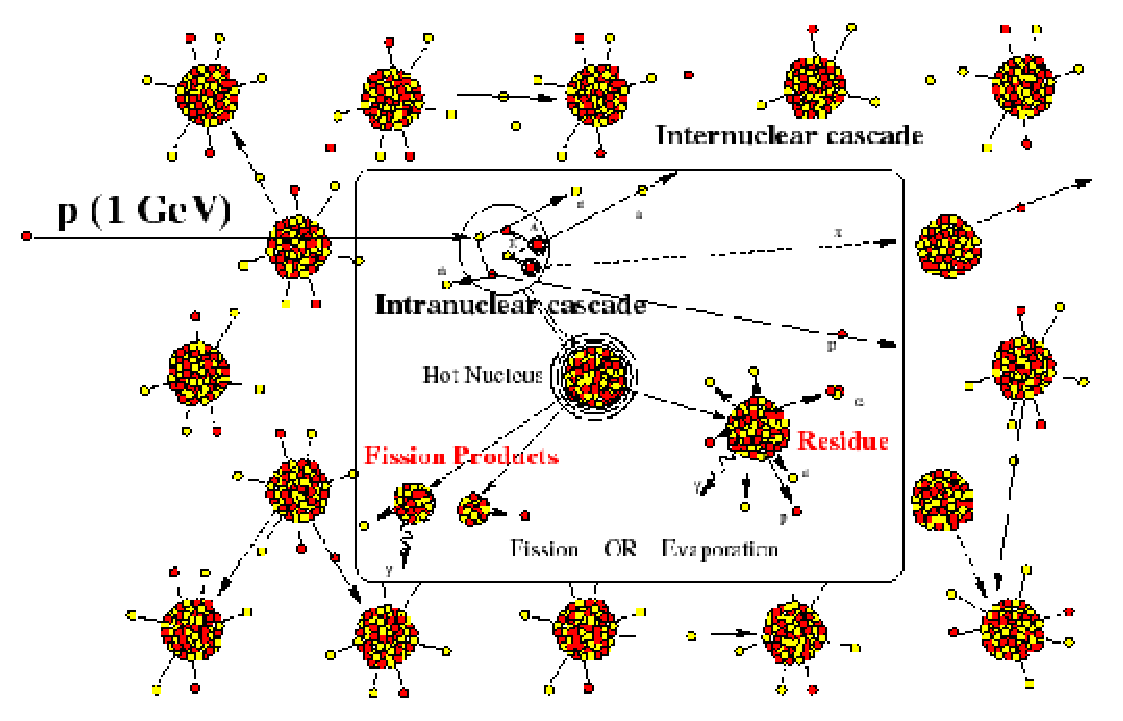
\includegraphics[scale=0.73]{images/cascade.eps}

\begin{comment}
\begin{textbox}
\section*{{\Huge {\sf INCL PARAMETERS}}}
%\section*{\textbf{\Large\color{udsubsect}\underline{INCL parameters}}}
{\color{udsect}
Li\`ege intra-nuclear cascade, {\sf INCL}, \cite{incl} requires \emph{only two free parameters}:
\begin{itemize}
\item potential depth, and
\item stopping time, $t_{stop}$, defined as the point in time when the cascade is
finished and evaporation starts:
\begin{equation}
t_{stop} = f_{stop}t_0 (A_{target}/208) ^{0.16}.
\end{equation}
\end{itemize}
Here $A_{target}$ is the target mass number, $t_0 = 70 fm/c$, and
$f_{stop}$ is a scaling factor for the stopping time \cite{g4incl}.
\vskip0.5cm

The number of parameters is kept low in order to have as much
\emph{predictive power} as possible.
}
% Good default value for this factor is $f_{stop}$ = 1.0

\end{textbox}
\end{comment}
%%%%%%%%%%%%%%%%%%%%%%%%%%%%%%%%%%%%%%%%%%%%%%%%%%%%%%%%%%%%%%%%%%%%%%%%%%%%%%%%%%
%\begin{textbox}


%\section*{{\Huge {\sf INCL}}}


%INCL is an intra-nuclear cascade model developed at the university of
%Li\`ege and CEA/Saclay.

%\end{textbox}
%%%%%%%%%%%%%%%%%%%%%%%%%%%%%%%%%%%%%%%%%%%%%%%%%%%%%%%%%%%%%%%%%%%%%%%%%%%%%%%
%\begin{textbox}


%\section*{{\Huge {\sf ABLA MODEL FOR EVAPO\-RATI\-ON AND FISSION}}}
%\section*{\color{udsect} ABLA}

%ABLA is a fission and evaporation code that is developed at GSI, Darmstadt.

%\end{textbox}
%%%%%%%%%%%%%%%%%%%%%%%%%%%%%%%%%%%%%%%%%%%%%%%%%%%%%%%%%%%%%%%%%%%%%%%%%%%%%%%%%
\begin{comment}
\begin{textbox}
\section*{{\Huge {\sf p(1.2 GeV) + Pb $\rightarrow$ n + X}}}
\vskip-1.5cm
\begin{figure}
\vskip3.5cm
{\Huge {\sf p(1.2 GeV) + Pb $\rightarrow$ n + X}}
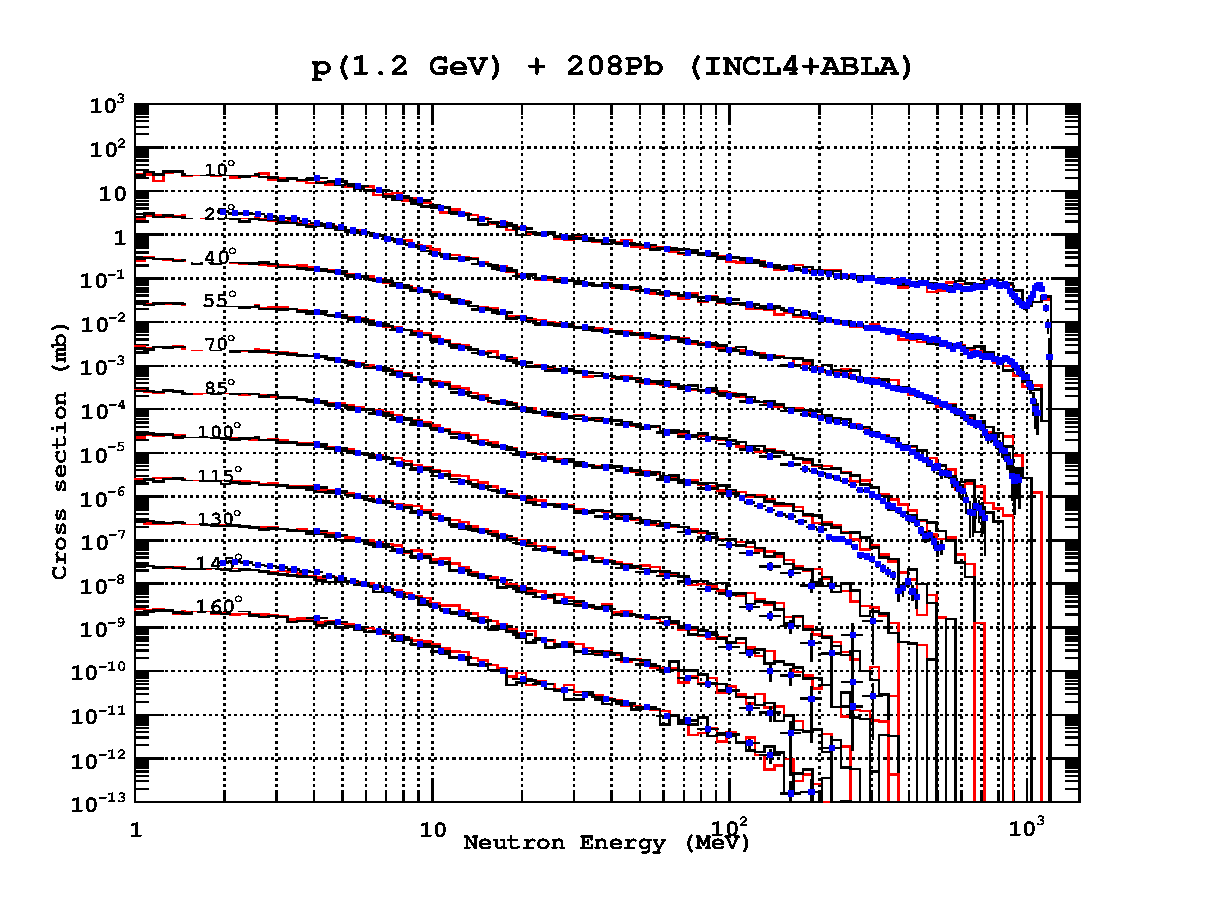
\includegraphics[scale=0.70]{images/lead.eps}
\label{fig:pPbdd1200MeV}
\end{figure}
\vskip-0.3cm
% FIXME linespread
{\Large {\sf {\linespread{1.5} Double-differential for neutron production cross section
    from {\sf Geant4} {\sf INCL} and {\sf ABLA} models. Neutron evaporation from {\sf ABLA} model is
    shown below E $\simeq$ 20 MeV. Black and red histograms are the
    results from the original {\sf FORTRAN} version and new {\sf C++} implementation, respectively. Blue data points are
    from Ref.~\cite{data}.}}}

\end{textbox}
\end{comment}
%%%%%%%%%%%%%%%%%%%%%%%%%%%%%%%%%%%%%%%%%%%%%%%%%%%%%%%%%%%%%%%%%%%%%%%%%%%%%%%%%%
\vspace{0.8cm}
\begin{textbox}
\section*{{\Huge {\sf GEANT4 PHYSICS LISTS}}}

A unique feature of {\sf Geant4} is to  
\emph{decouple physics models, cross sections, and processes}
using abstract interfaces, and manage the usage of different options with so-called the physics lists.


\begin{itemize}
{\color{udsect}
\item Physics lists allow users to find good balance between various goals (e.g. CPU
time requirements vs. accuracy of results).
}
\item Also, users can run their simulation using different physics model
configurations and compare the results.
%\item Allow alternative implementations

\item Further, the {\sf Geant4} physics system can be easily extended.
%\item Each application must define explicitly what physics
%configuration to use
\end{itemize}

%\begin{comment}
%The options are: use a \emph{reference physics list} or build your own.
%\begin{itemize}
%\item Everything related to physics is a \emph{process}.
%\item Each particle has a pointer to its \emph{particle definition}.
%\item Particle definition has exactly one \emph{process manager}.
%\item Process manager keeps track of different processes assigned to the particle.
%\item Process has cross section and a model associated with it.
%\end{itemize}
%\end{comment}
\end{textbox}

%%%%%%%%%%%%%%%%%%%%%%%%%%%%%%%%%%%%%%%%%%%%%%%%%%%%%%%%%%%%%%%%%%%%%%%%%%%%%%%%%%

%%%%%%%%%%%%%%%%%%%%%%%%%%%%%%%%%%%%%%%%%%%%%%%%%%%%%%%%%%%%%%%%%%%%%%%%%%%%%%%%%%
%\vspace{-5cm}
\vspace{0.4cm}
\begin{textbox}

\section*{{\Huge {\sf  A NEW PHYSICS LIST}}}

{\color{udsect}

We have implemented a new physics list called {\sf QGSP\_\-INCL\-ABLA} with
spallation physics in mind. 
}

\vspace{1cm}
This list uses {\sf INCL/ABLA} models for proton,
neutron and pion inelastic interactions in the energy range 0 - 3
GeV.
\vskip1cm
In this energy range {\sf INCL/ABLA} is the only model used for the
%aforementioned 
these processes.

\end{textbox}

%%%%%%%%%%%%%%%%%%%%%%%%%%%%%%%%%%%%%%%%%%%%%%%%%%%%%%%%%%%%%%%%%%%%%%%%%%%%%%%%%%
%\begin{textbox}
\vspace{2cm}
\section*{{\Huge {\sf FRAGMENT YIELD}}}
\vspace{-1cm}
%Fragments produced in reaction: p(1 GeV) + Pb
\begin{center}

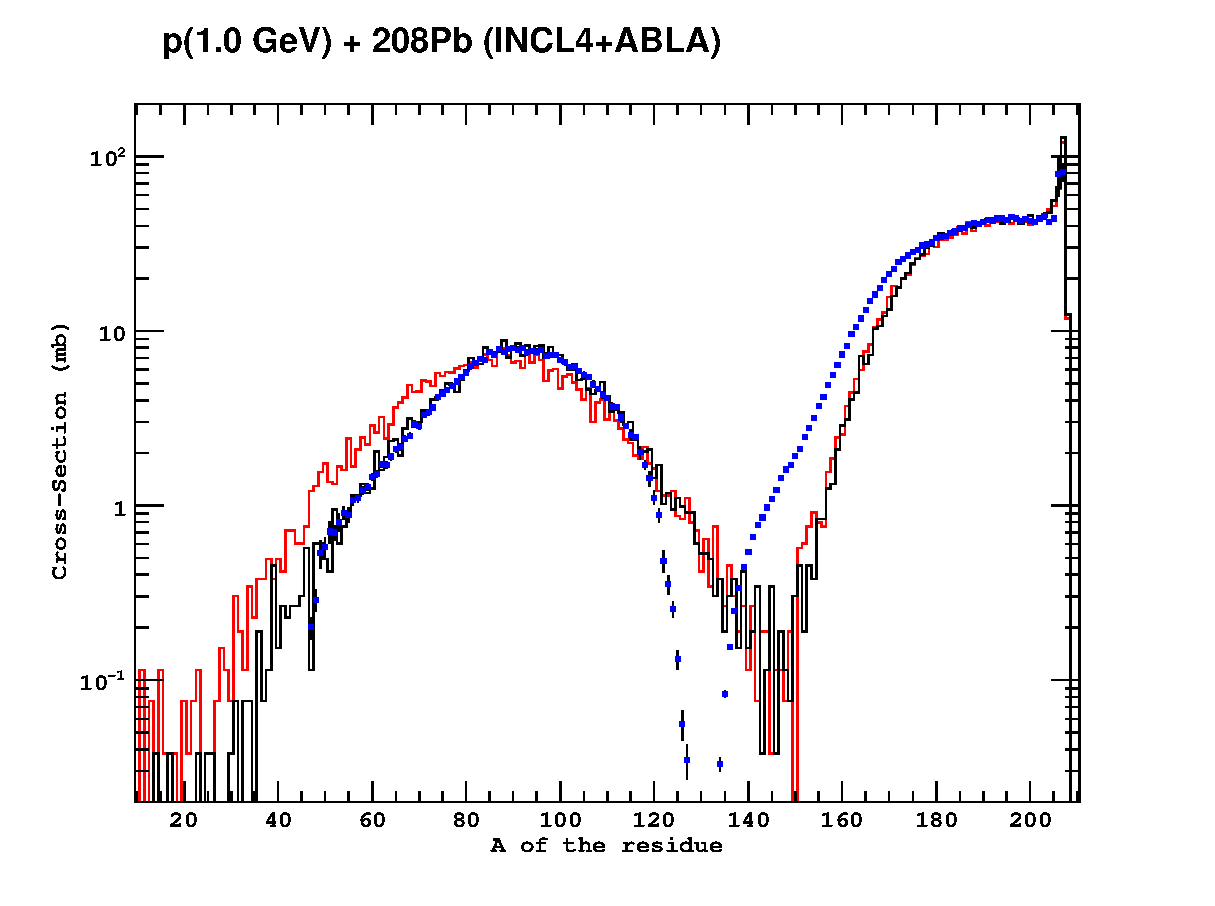
\includegraphics[scale=0.70]{images/fragments.eps}

\vspace{1.5cm}
%Isotope production:
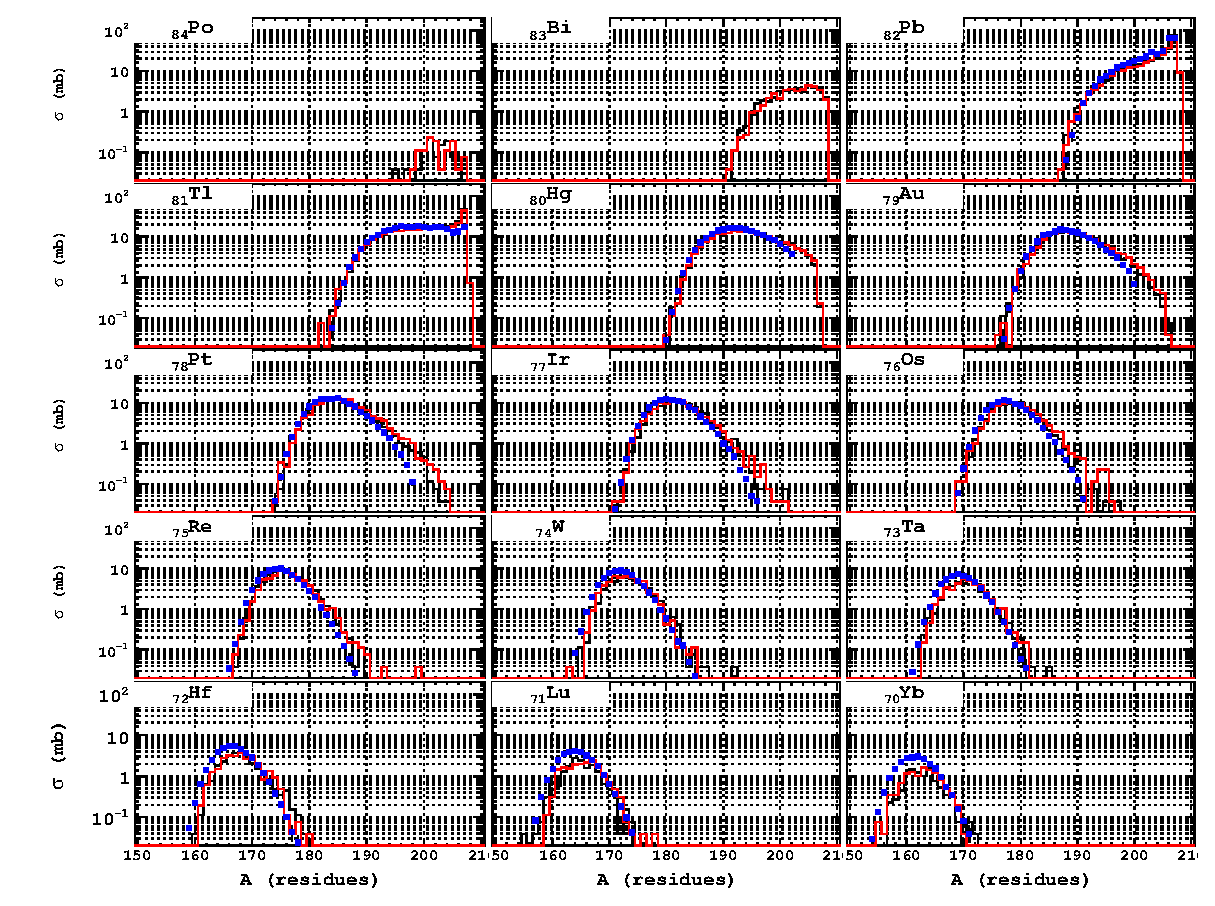
\includegraphics[scale=0.60]{images/pPbIsotopes.eps}
{\Large {\sf {\linespread{1.0} Fragment production of the {\sf INCL} and {\sf ABLA} \cite{abla} models. Black and red histograms are the
    results from the original {\sf FORTRAN} version and new {\sf C++} implementation, respectively.}}}
\end{center}
%\end{textbox}
%%%%%%%%%%%%%%%%%%%%%%%%%%%%%%%%%%%%%%%%%%%%%%%%%%%%%%%%%%%%%%%%%%%%%%%%%%%%%%%%%%

%%%%%%%%%%%%%%%%%%%%%%%%%%%%%%%%%%%%%%%%%%%%%%%%%%%%%%%%%%%%%%%%%%%%%%%%%%%%%%%%%%
%\begin{textbox}

\vspace{0.5cm}
\section*{{\Huge {\sf NEUTRON PRODUCTION}}}
\vspace{-1.6cm}
%Neutron production:
\begin{center}
%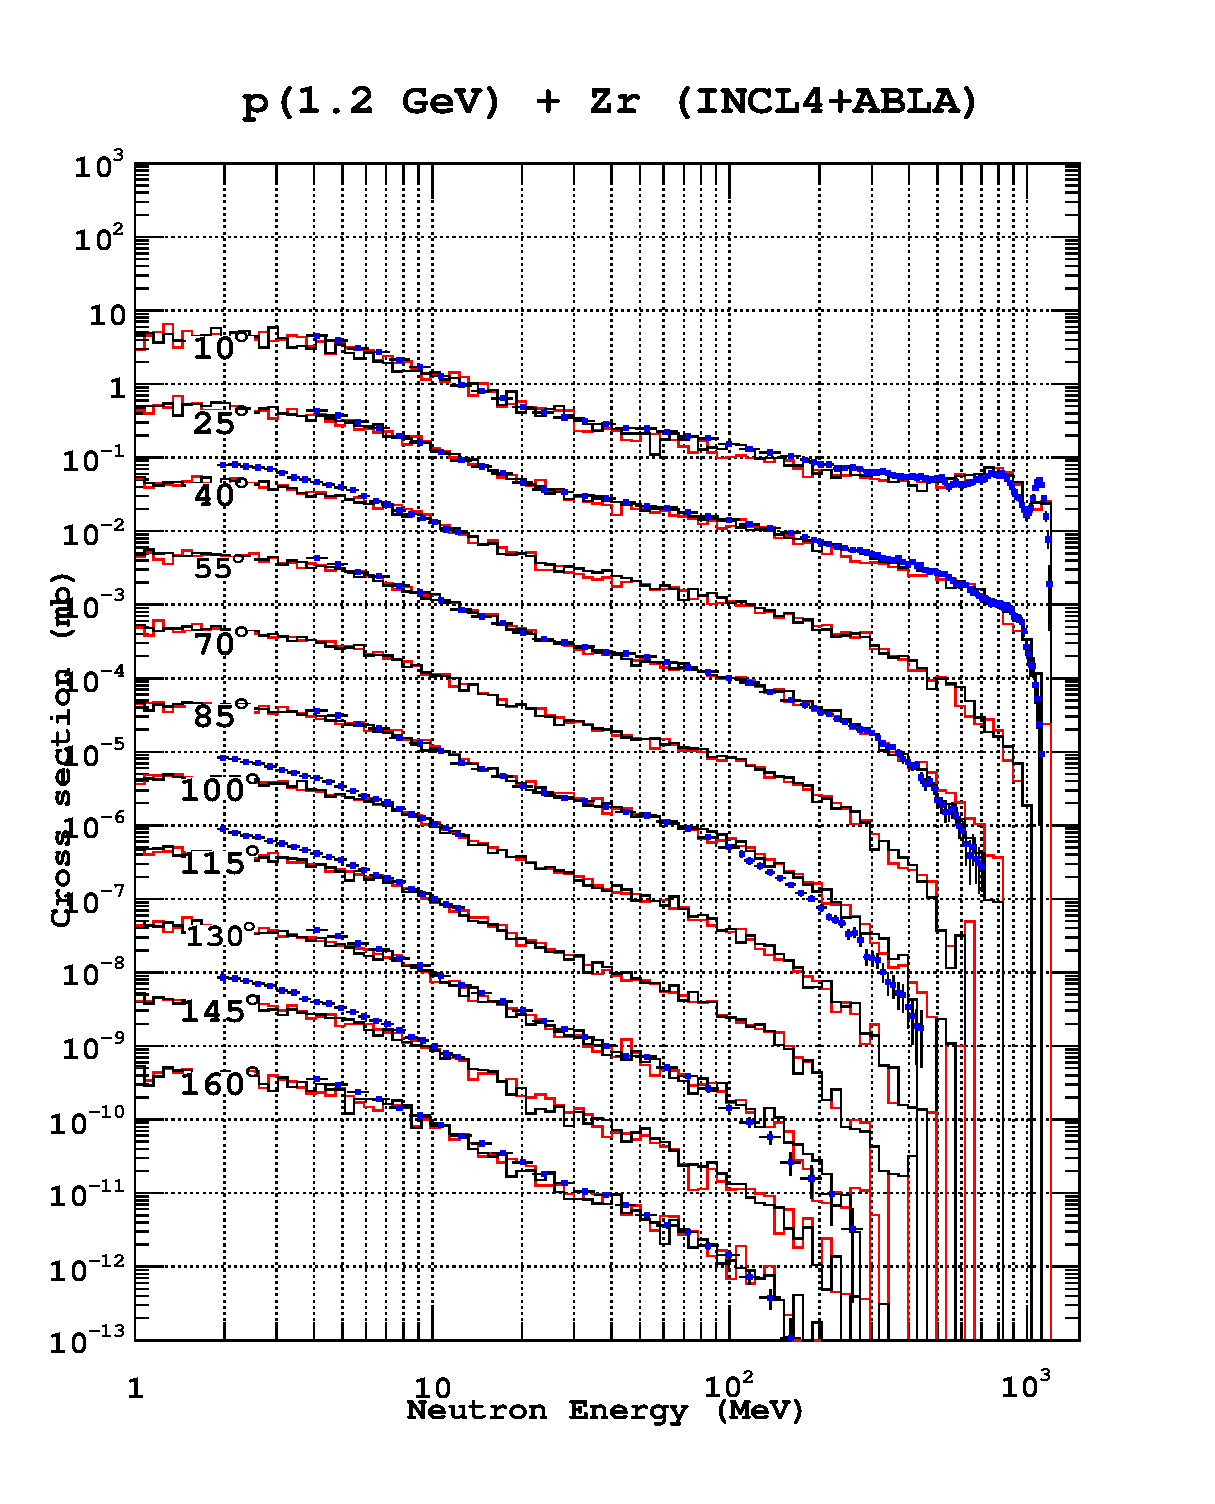
\includegraphics[scale=0.5]{images/zirkonium.eps}
%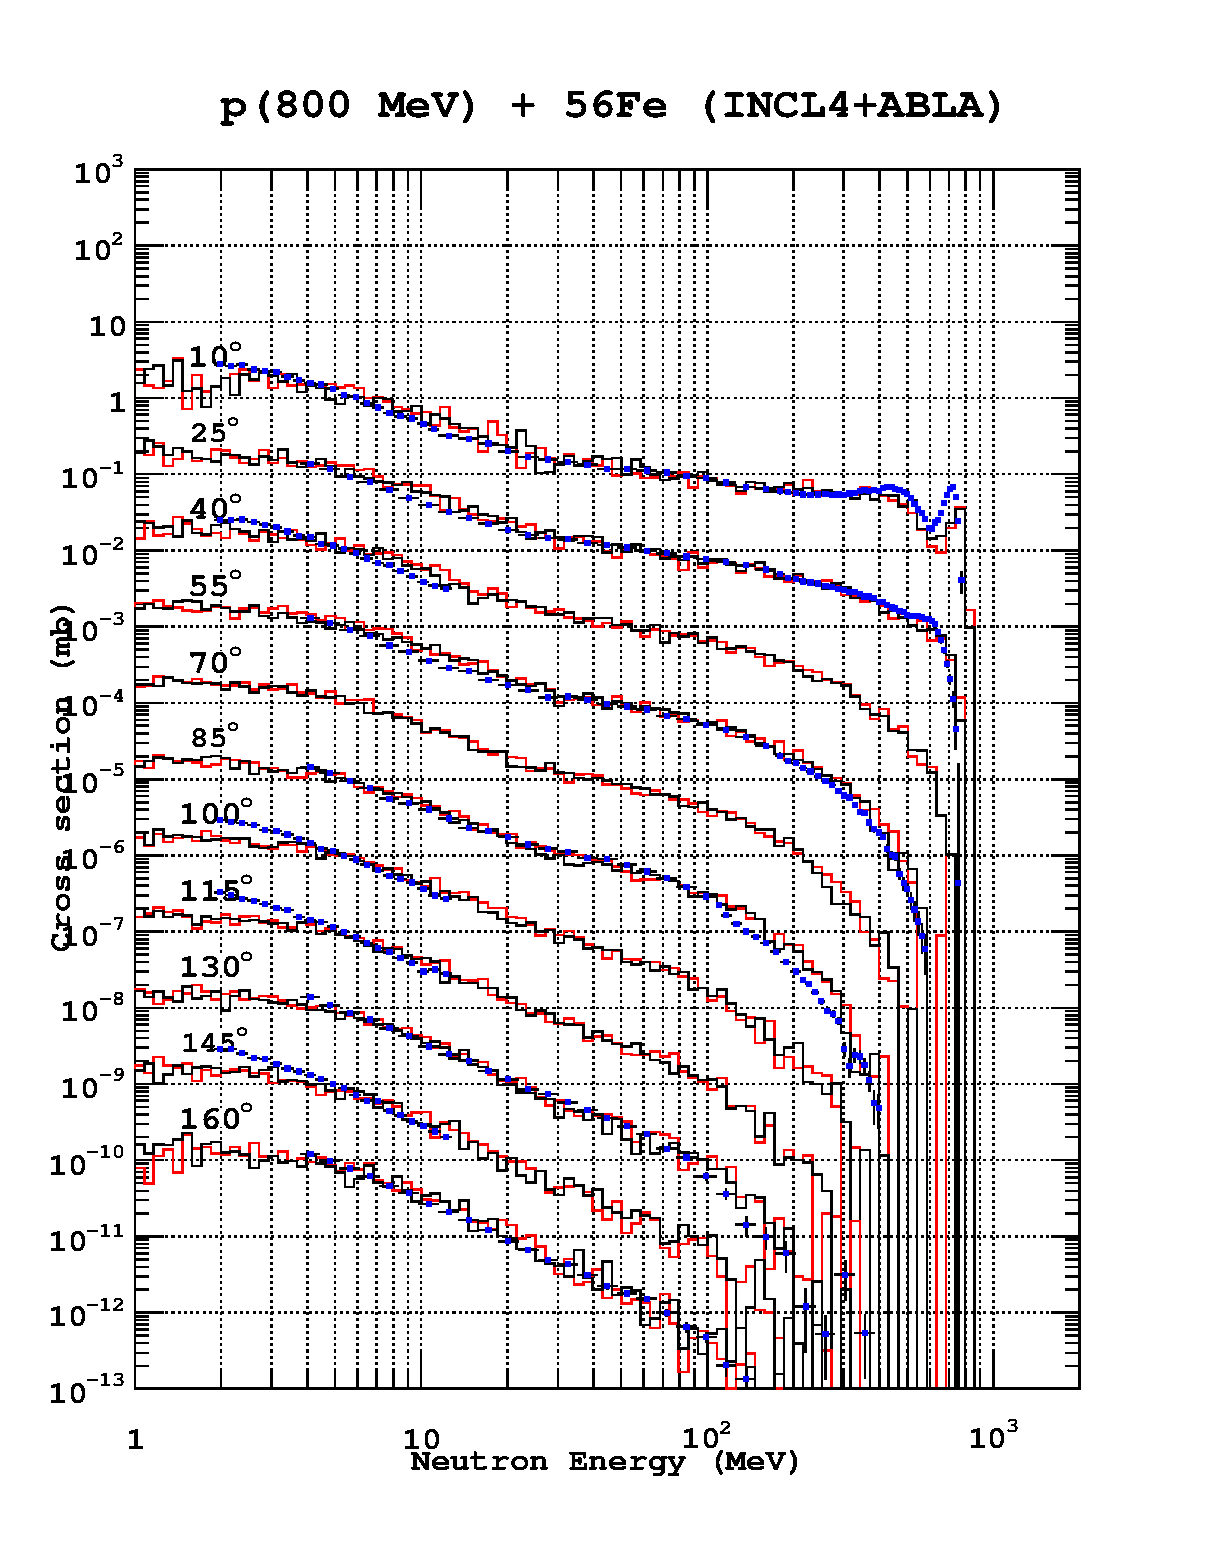
\includegraphics[scale=0.5]{images/iron.eps}
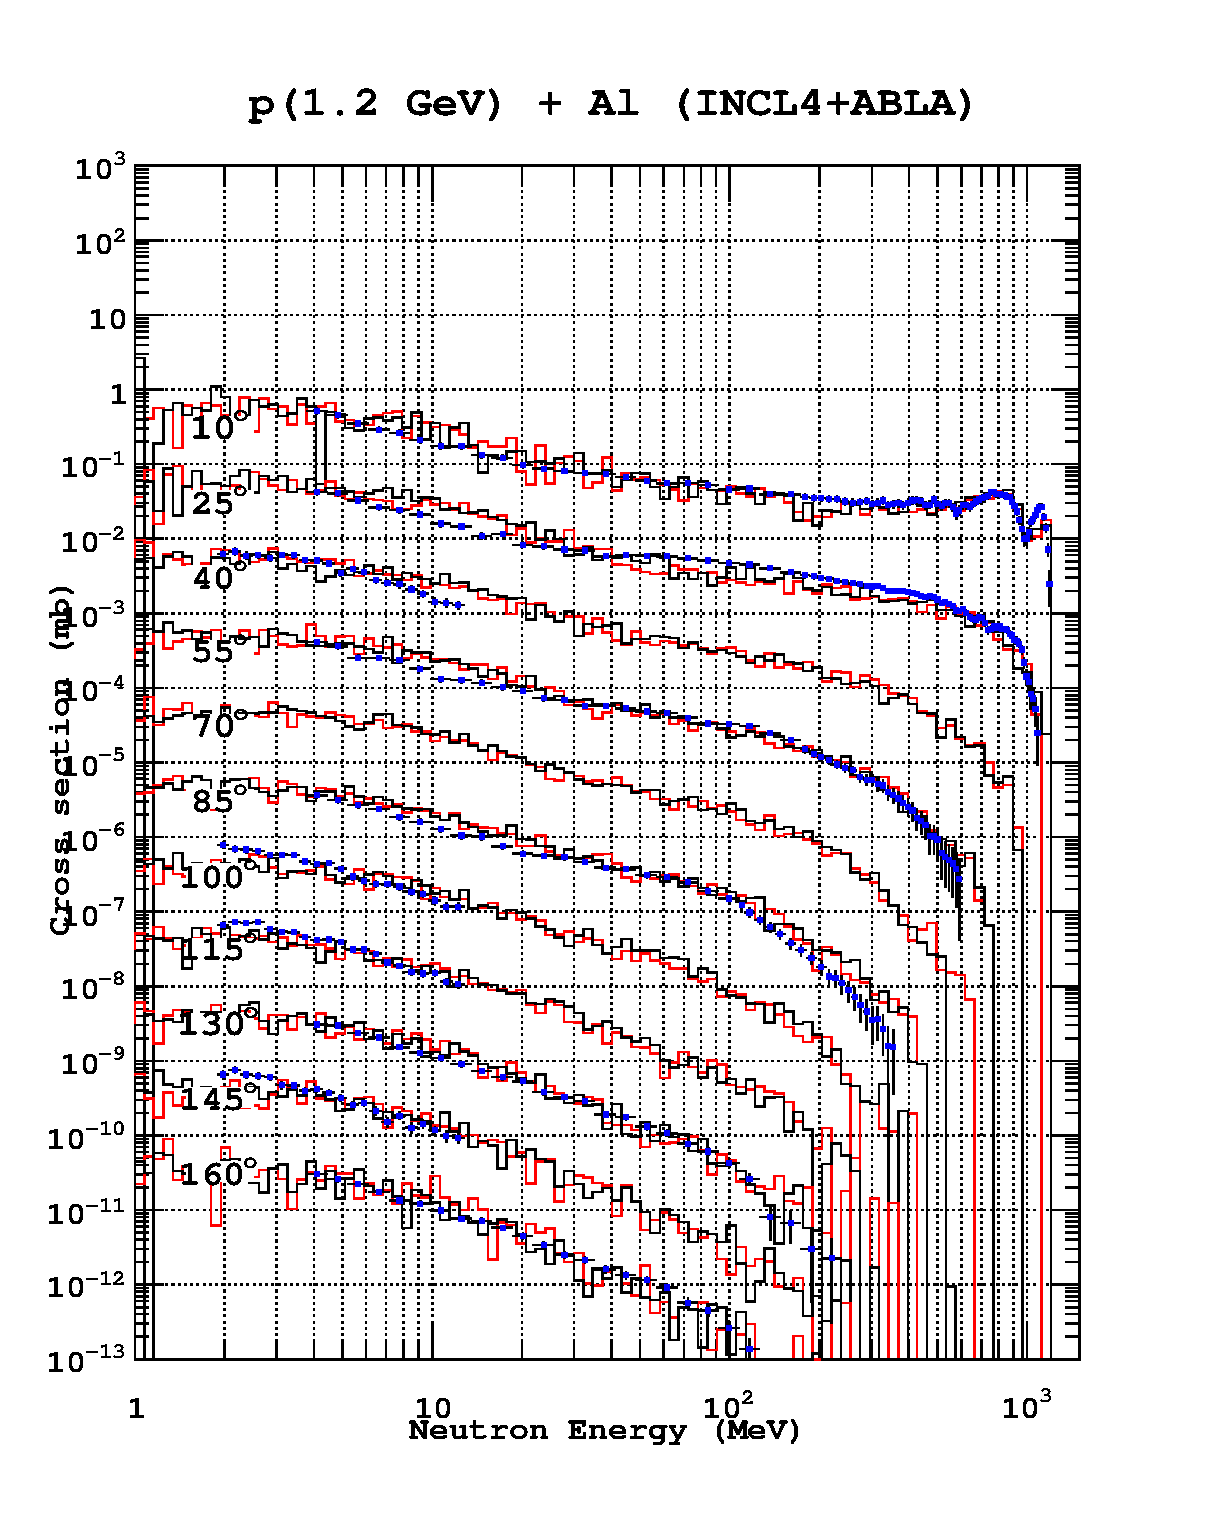
\includegraphics[scale=0.69]{images/aluminum.eps}
{\Large {\sf {\linespread{1.0} Double-differential for neutron production cross section
    from {\sf Geant4} {\sf INCL} and {\sf ABLA} models. Black and red histograms are the
    results from the original {\sf FORTRAN} version and new {\sf C++} implementation, respectively. Data points are
    from Ref.~\cite{data}.}}}
\end{center}
%\end{textbox}
%%%%%%%%%%%%%%%%%%%%%%%%%%%%%%%%%%%%%%%%%%%%%%%%%%%%%%%%%%%%%%%%%%%%%%%%%%%%%%%%%%

\vspace{5cm}

\begin{textbox}
\section*{{\Huge {\sf LIGHT TARGETS}}}

{\color{udsect}
We have introduced a cut to choose between {\sf ABLA} and Fermi break-up for light targets.
So, \emph{{\sf INCL} can now be used with the {\sf Geant4} Fermi break-up model}.
}

\vspace{1cm}
Currently, {\sf INCL} interface provides Fermi break-up \cite{g4incl} for
remnant nuclei lighter than A = 13 and {\sf ABLA} for heavier elements.
\end{textbox}

\begin{center}
{\Huge {\sf 1 GeV PROTON  ON CARBON}}

\vspace{1cm}
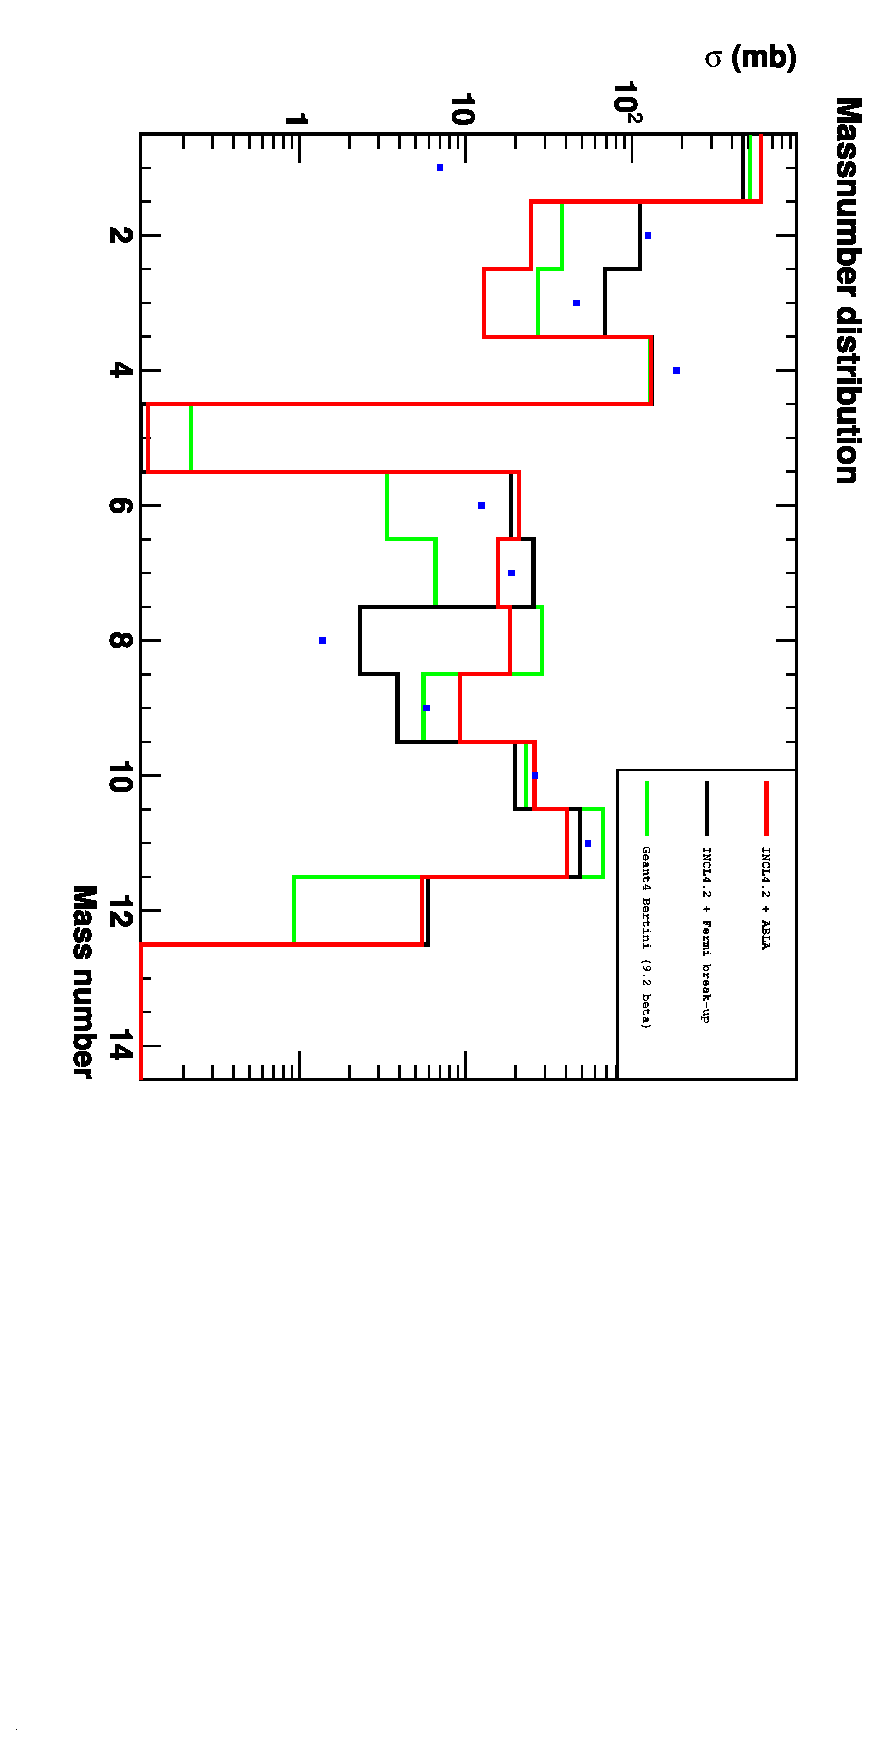
\includegraphics[scale=0.72,angle=90]{images/masses.eps}
\end{center}

\begin{textbox}
\section*{{\Huge {\sf CARBON PROJECTILES}}}
An ongoing work is to improve of the physics models for the treatment of 
light ion beams up to Carbon.

\vspace{1cm}
{\color{udsect}
Carbon beams are of particular interest for medical applications of {\sf
Geant4}, and recently, a Carbon projectile support has been added to the {\sf INCL}
cascade. 

%{\tt NOTE: CARBON FIGS PRODUCED USING BUGGY CODE. THEY WILL NOT BE
%PART OF THE POSTER}
%\begin{center}
%{\Huge {\sf C(400 MeV/nucleon) + Cu}}
%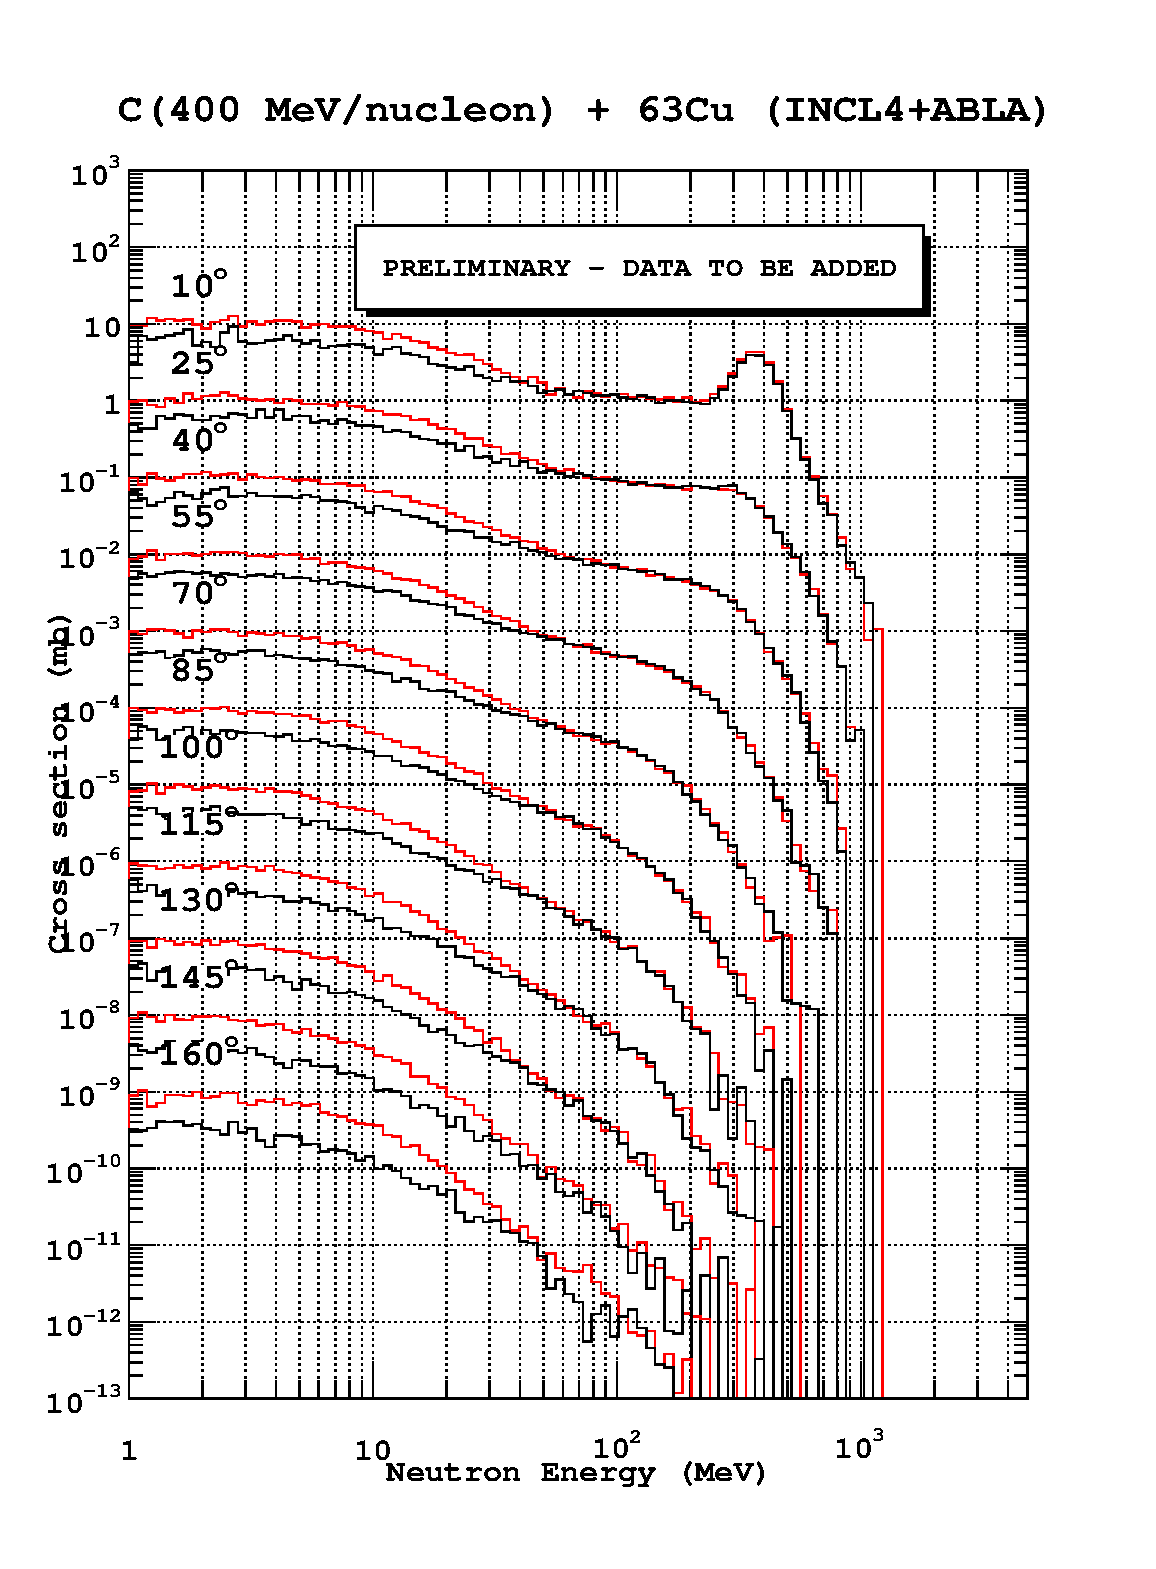
\includegraphics[scale=0.6,angle=0]{images/carbonCopper.eps}
%\end{center}
%\begin{center}
%{\Huge {\sf C(400 MeV/nucleon) + Cu}}
%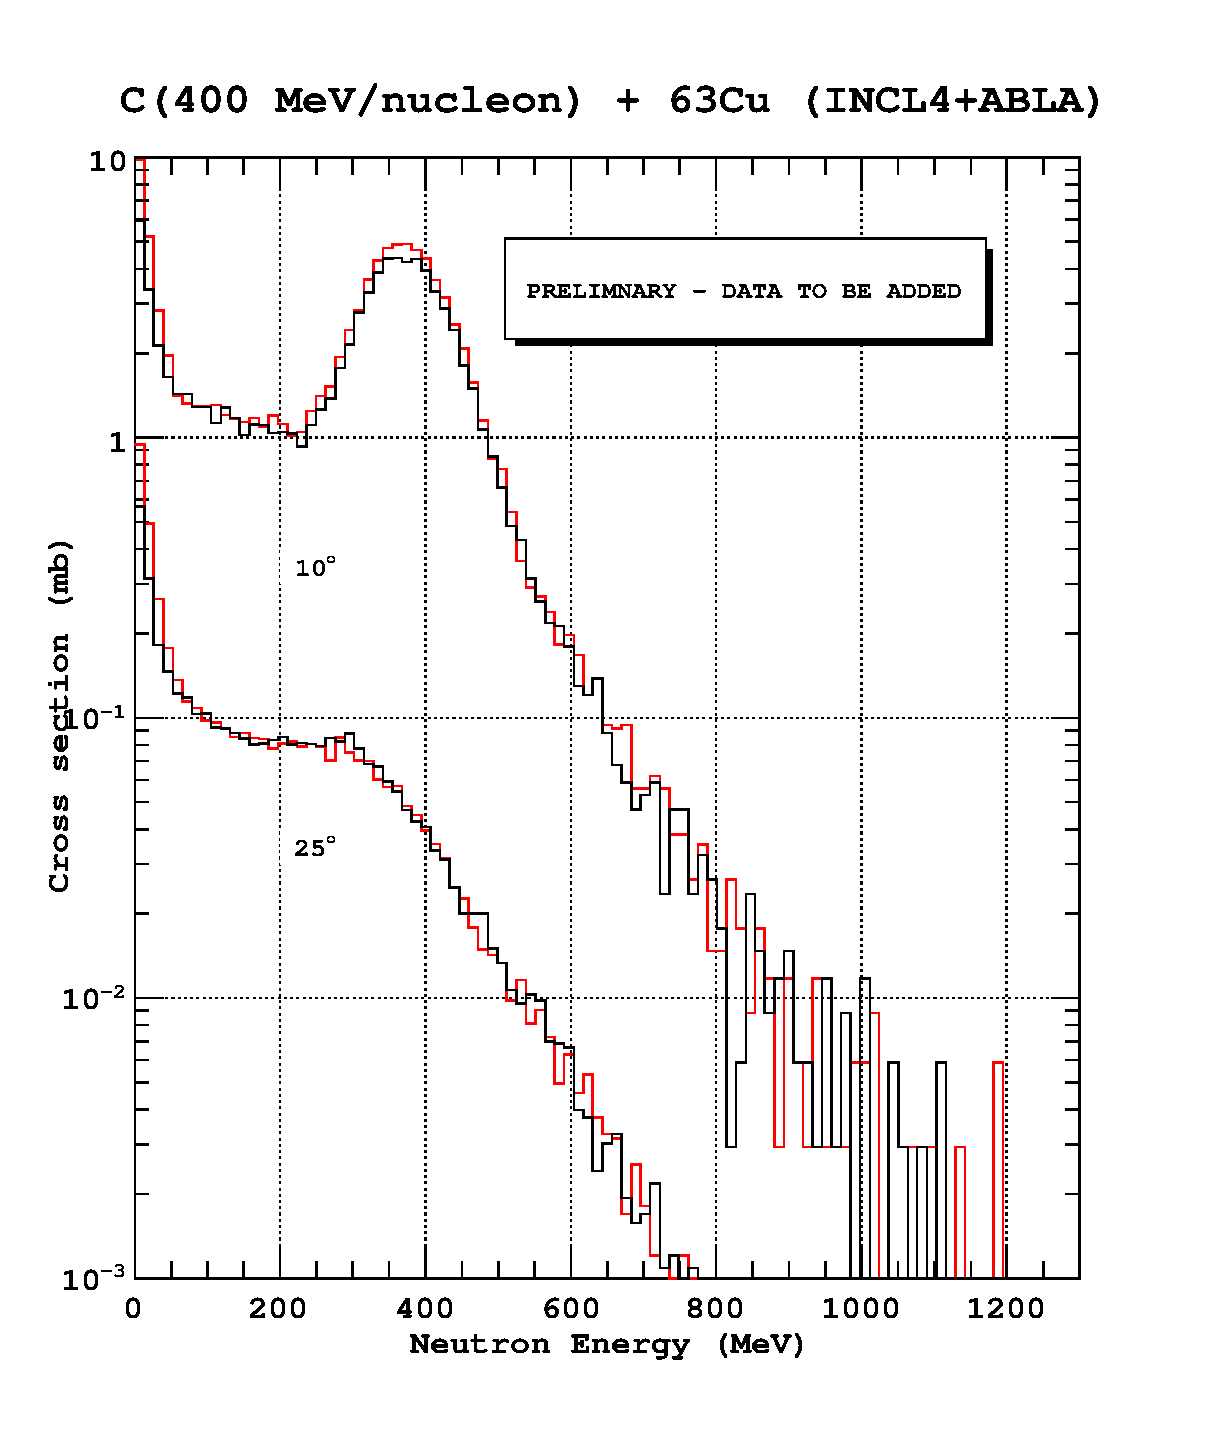
\includegraphics[scale=0.6,angle=0]{images/carbonCopperLin.eps}
%\end{center}
}
%\vspace{-1cm}
\end{textbox}


\begin{comment}
\begin{textbox}
\section*{{\Huge {\sf ABLA EVAPORATION}}}
{\color{udsect}
The ablation code {\sf ABLA} \cite{abla} for evaporation and fission modeling is developed at GSI, Darmstadt.
\vskip0.5cm

The probabilities for emission of particle type $j$ = \{$p$, $n$, $\alpha$\}
are calculated using formula:
\begin{equation}
W_j(N,Z,E) = \frac{\Gamma_j(N,Z,E)}{\sum_k\Gamma_k(N,Z,E)},
\label{eqn:probabilities}
\end{equation}
where $N$ is neutron
number, $Z$ charge number and $E$ excitation energy.
\vskip0.5cm

The emission width, $\Gamma_j$, for particle $j$ is defined as:
\index{emission width}
\begin{equation}
\Gamma_j = \frac{1}{2 \pi \rho_c(E)} \frac{4 m_j R^2}{\hbar^2} T_j^2 \rho_j(E - S_j - B_j),
\label{eqn:emissionwidth}
\end{equation}
where:
\begin{itemize}
\item $\rho_c(E)$ and $\rho_j(E - S_j - B_j)$ are the level densities
of the compound nucleus and the exit channel, respectively.
\item $B_j$ the height of the Coulomb barrier,
\item $S_j$ the separation energy,
\item $R$ the radius,
\item $T_j$ the temperature of the remnant nucleus after
emission, and
\item $m_j$ the mass of the emitted particle.
\end{itemize}
}
\end{textbox}
\end{comment}
%%%%%%%%%%%%%%%%%%%%%%%%%%%%%%%%%%%%%%%%%%%%%%%%%%%%%%%%%%%%%%%%%%%%%%%%%%%%%%%%%%

%\section*{{\Huge {\sf }}}
%{\Huge {\sf p(0.8 GeV) + Pb $\rightarrow$ n + X}}

%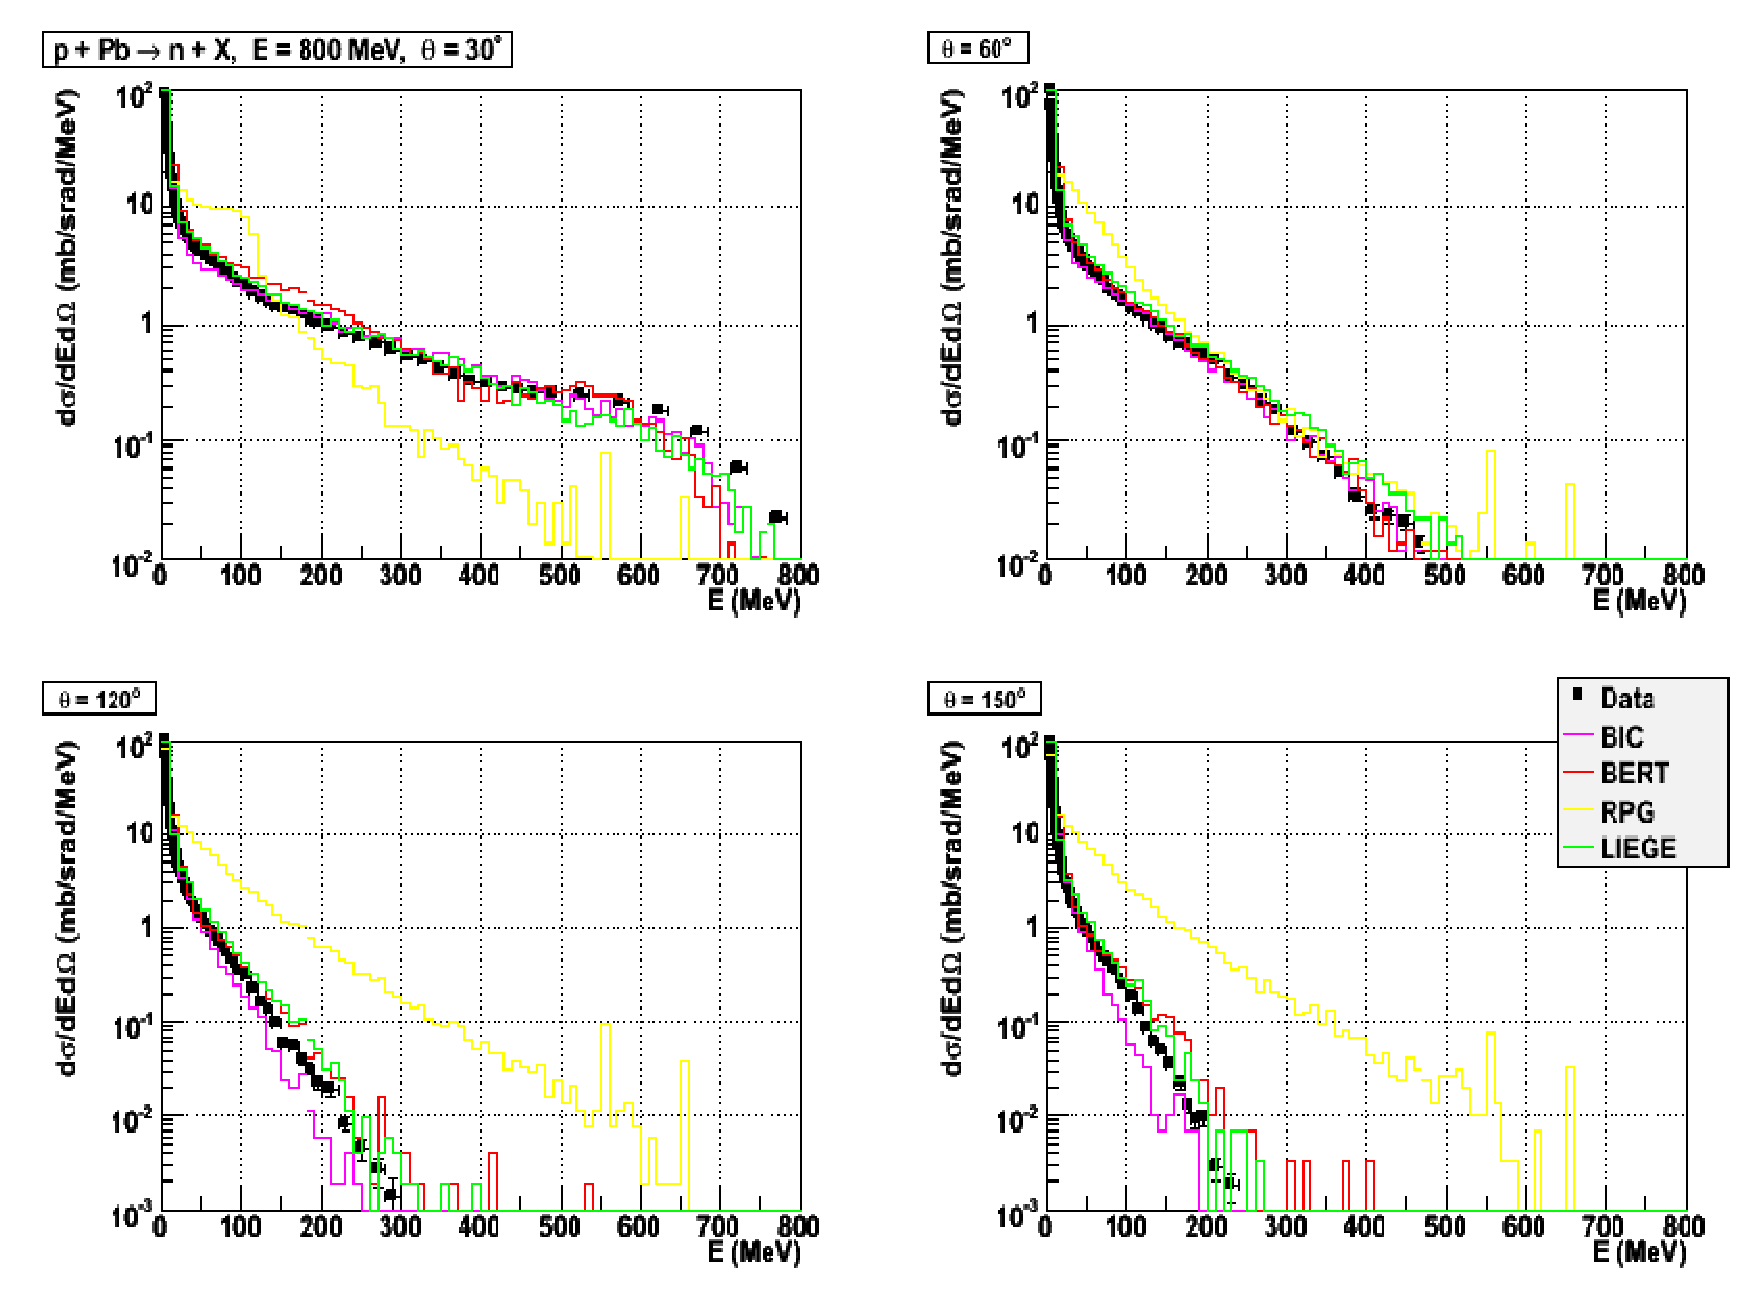
\includegraphics[scale=0.45]{images/vladimir.eps}
%{\Large {\sf Comparison of various models in {\sf Geant4}. Li\`ege cascade together with ABLA (label ``LIEGE'') is compared against experimental data and other {\sf Geant4} models (BIC, BERT, RPG).
% {\sf INCL/ABLA} simulation is in good agreement with experimental data. (\emph{Courtesy of
%    V. Ivantchenko, Geant4 collaboration}.)}}

%%%%%%%%%%%%%%%%%%%%%%%%%%%%%%%%%%%%%%%%%%%%%%%%%%%%%%%%%%%%%%%%%%%%%%%%%%%%%%%%%%%
%\begin{textbox}


%\section*{{\Huge {\sf ACKNOWLEDGEMENTS}}}

%This work has been a collaborative effort with the original developers from
%Li\`ege University, GSI and CEA. We acknowledge the help from J.~Cugnon,
%A.~Boudard, Y.~Yariv, S.~Leray, C.~Schmidt and K.~H.~Schmidt
%on reimplementing the original {\sf FORTRAN} codes in {\sf C++} language.

%\end{textbox}
%%%%%%%%%%%%%%%%%%%%%%%%%%%%%%%%%%%%%%%%%%%%%%%%%%%%%%%%%%%%%%%%%%%%%%%%%%%%%%%%%%%
%\vskip2cm
%\begin{textbox}
\addcontentsline{toc}{section}{References}
%\section*{{\Huge {\sf REFERENCES}}}
{\Large

%\bibliographystyle{abbrv}
%\bibliography{latex_poster}
%\bibliographystyle{unsrt} 
\begin{thebibliography}{9}

\bibitem{incl} A. Boudard et al., \emph{Intranuclear cascade model for
    a comprehensive description of spallation reaction data}, Phys.
  Rev. C66 (2002) 044615
\bibitem{g4} \emph{Geant4 collaboration website} \\ {\tt http://\-cern.ch/\-geant4}
\bibitem{pk08bProceedings}
A. Heikkinen, P. Kaitaniemi, and A. Boudard,
{\em Implementation of INCL4 cascade and ABLA evaporation codes in Geant4},
Journal of Physics: Conference Series 119 (2008) 032024, 
{\sf [doi:10.1088/1742-6596/119/3/032024]}

\bibitem{abla} J. Benlliure et al., \emph{Calculated nuclide
    production yields in relativistic collisions of fissile nuclei},
  Nuc. Phys. A628 (1998) 458
\bibitem{g4incl} \emph{Geant4 Physics Reference Manual: INCL~4.2 Cascade and ABLA~V3 Evaporation with Fission} 
%\\ {\tt http://geant4.web.cern.ch/\-geant4/\-UserDocumentation/\-UsersGuides/\-PhysicsReferenceManual/\-html/\-node185.html}

\bibitem{data} X.Ledoux et al., \emph{Spallation Neutron Production by
  0.8, 1.2, and 1.6 GeV Protons on Pb Targets} Phys. Rev. Lett. 82
  (1999)

%\bibitem{pk09aCollaboration}
%P. Kaitaniemi and A. Heikkinen with Geant4 Collaboration
%{\tt http://www.geant4.org}{http://www.geant4.org}

%\bibitem{fp} P. Kaitaniemi, A. Heikkinen, \emph{Implementing INCL4
%    hadronic cascade and ABLA de-excitation codes in Geant4},
%  Proceedings of the 41th Annual Meeting of the Finnish Physical
%  Society (2007)

%\bibitem{pk08aProceedings}
%P. Kaitaniemi and A. Heikkinen,  
%{\em INCL4 cascade and ABLA evaporation codes in Geant4},
%Proceedings of the XLII annual conference of the Finnish Physical Society, 
%                 March 27-29 2008, Turku, Finland. 
%                 Report Series in Physics L 31, University of Turku, 2008.


%\bibitem{carbone}
%D.L. Olson et al.,
%{\em Factorization of fragment-production cross sections in relativistic heavy-ion collisions},
%Phys. Rev. C28, 1602 (1983)
%{\sf [doi:10.1103/PhysRevC.28.1602]}

\end{thebibliography}


%\end{textbox}
%%%%%%%%%%%%%%%%%%%%%%%%%%%%%%%%%%%%%%%%%%%%%%%%%%%%%%%%%%%%%%%%%%%%%%%%%%%%%%%%%%%
}
\end{multicols}

\end{center}
\end{document}
